\clearpage

\section{Opaque without Survivability - Reference Network} \label{Reference_Network}

In this case study we focus on the opaque case without survivability for the reference network.
The opaque transport mode performs OEO (optical-electric-optical) conversions on each intermediate node from the source to the destination node.
One advantage of this mode of transport is that it eliminates accumulation of physical impairments, and allows optimum grooming by performing grooming at each node.


\subsection{Dimensioning using ILP}
\begin{tcolorbox}	
\begin{tabular}{p{2.75cm} p{0.2cm} p{10.5cm}} 	
\textbf{Student Name}  &:& Tiago Esteves    (October 03, 2017 - )\\
\end{tabular}
\end{tcolorbox}

\vspace{11pt}
In this section we will do the dimensioning of the network mentioned in the first subsection to calculate the value of your CAPEX, for this we will use the ILP model describe in section \ref{ILP_Opaque_Survivability} and we can get the best possible solution.
In the initial subsection will be described the network cost where all the formulas and calculations necessary to obtain the CAPEX of the network will be mentioned.
Finally, in the last subsection, the results obtained through the described model will be presented.

\subsubsection{Network costs}\label{Net_Costs}

In this phase the results will be presented to calculate the CAPEX of the reference network.
The value of the CAPEX of the network will be calculated based on the costs of the equipment present in the table \ref{table_cost_opaque}.
In addition to the equipment costs we will also use the parameter "span", which in this case will have a value of 100, because this value is used to calculate the number of optical amplifiers required in the network using Equation \ref{amplifiers}.\\

To know the value of CAPEX it is necessary to know the value of the cost of the links and the cost of the nodes.
To calculate the cost of the nodes, the sum of the costs of the optical and electrical node is made. For this case the value of the optical cost is zero only needing to know the electric cost of the nodes that is given by equation \ref{electricalCostOpaque}.

\begin{equation}
C_{exc} = \left(\gamma_{e0}\times N\right) + \gamma_{e1} \times \left(T_1 + \left(2 \times w^0 \times \tau \right)\right)
\label{electricalCostOpaque}
\end{equation}

\begin{itemize}
\item{$C_{exc}$		$\rightarrow$	Electrical ports cost}
\item{$\gamma_{e0}$	$\rightarrow$	EXC cost in euros}
\item{$N$			$\rightarrow$	Number of nodes}
\item{$\gamma_{e1}$	$\rightarrow$	EXC port cost in euros}
\item{$T_1$         $\rightarrow$   Total unidirectional traffic}
\item{$w^0$			$\rightarrow$	Total number of optical channels}
\item{$\tau$		$\rightarrow$	Traffic per port}
\end{itemize}

\vspace{11pt}

To calculate the cost of the Links we will use the equation \ref{linkCosts}.

\begin{equation}
C_L = \left(2 \times \gamma_0^{OLT} \times L\right) + \left(2 \times \gamma_1^{OLT} \times \tau \times W\right) + \left(N^R \times c^R\right)
\label{linkCosts}
\end{equation}	
	
\begin{itemize}
\item{$C_L$				$\rightarrow$	Links cost}
\item{$\gamma_0^{OLT}$	$\rightarrow$	OLT cost in euros}
\item{$L$				$\rightarrow$	Number of unidirectional links}
\item{$\gamma_1^{OLT}$	$\rightarrow$	Transponder cost in euros}
\item{$W$             $\rightarrow$	    Total number of optical channels}
\item{$N^R$				$\rightarrow$	Total number of optical amplifiers}
\item{$c^R$				$\rightarrow$	Optical amplifiers cost in euros}
\end{itemize}

\subsubsection{ILP Results}

To perform the calculations using the implementation of the models described in section \ref{ILP_Opaque_Survivability} it is necessary to use a mathematical software tool. For this we will use MATLAB which is ideal for dealing with linear programming problems and can call the LPsolve through an external interface. \\

\textbf{Scenario 1: Reference Network Low Traffic} \label{Scenario1_opaque} \\

In this scenario we used the table \ref{table_ref_net}. In the table \ref{result_ILP1_reference} we can see the values calculated through MatLab and using the values indicated in table \ref{table_cost_opaque} we can finally calculate the CAPEX value.
\begin{table}[h!]
\centering
\begin{tabular}{|| c | c||}
 \hline
 Number of optical channels & Value \\
 \hline\hline
 in the link (1,2) & 1 \\
 in the link (1,3) & 1 \\
 in the link (2,3) & 1 \\
 in the link (2,4) & 2 \\
 in the link (3,5) & 1 \\
 in the link (4,5) & 1 \\
 in the link (4,6) & 2 \\
 in the link (5,6) & 2 \\
 \hline
\end{tabular}
\caption{Table with results}
\label{result_ILP1_reference}
\end{table}

Using equation \ref{linkCosts} : \\
$C_L$ = $($2 * 15 000 * 8$)$ + $($2 * 5 000 * 100 * 11$)$ + $($33 * 4 000$)$ \\
$C_L$ = \textbf{11 372 000 \euro} \\


Using equation \ref{electricalCostOpaque} : \\
$C_{exc}$ = $($6 * 10 000$)$ + 1 000 * $($1 000 + $($2 * 11 * 100$)$ $)$ \\
$C_N$ = $C_{exc}$ = \textbf{3 260 000 \euro} \\

$CAPEX$ = 11 372 000 + 3 260 000 \\
$CAPEX$ = \textbf{14 632 000 \euro}\\

Through image \ref{scriptopaque_surv_ref_low} we can see that the previous ILP based calculations are correct.
\begin{figure}[h!]
\centering
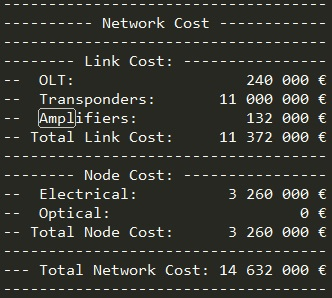
\includegraphics[width=8cm]{sdf/opaque/figures/script_opaque_surv_ref_low}
\caption{The ILP script used with the network cost.}
\label{scriptopaque_surv_ref_low}
\end{figure}


\textbf{Scenario 2: Reference Network High Traffic} \label{Scenario2_opaque} \\

In this scenario we used again the table \ref{table_ref_net}. In the table \ref{result_ILP2_reference} we can see the values calculated through MatLab and using the values indicated in table \ref{table_cost_opaque} we can finally calculate the CAPEX value.
\begin{table}[h!]
\centering
\begin{tabular}{|| c | c||}
 \hline
 Number of optical channels & Value \\
 \hline\hline
 in the link (1,2) & 4 \\
 in the link (1,3) & 4 \\
 in the link (2,3) & 4 \\
 in the link (2,4) & 19 \\
 in the link (3,5) & 9 \\
 in the link (4,5) & 5 \\
 in the link (4,6) & 16 \\
 in the link (5,6) & 14 \\
 \hline
\end{tabular}
\caption{Table with results}
\label{result_ILP2_reference}
\end{table}

Using equation \ref{linkCosts} : \\
$C_L$ = $($2 * 15 000 * 8$)$ + $($2 * 5 000 * 100 * 75 $)$ + $($33 * 4 000$)$ \\
$C_L$ = \textbf{ 75 372 000 \euro} \\

Using equation \ref{electricalCostOpaque} : \\
$C_{exc}$ = $($6 * 10 000$)$ + 1 000 * $($10 000 + $($2 * 75 * 100$)$ $)$ \\
$C_N$ = $C_{exc}$ = \textbf{25 060 000 \euro} \\

$CAPEX$ = 75 372 000 + 25 060 000 \\
$CAPEX$ = \textbf{100 432 000 \euro}\\

Through image \ref{scriptopaque_surv_ref_high} we can see that the previous ILP based calculations are correct.
\begin{figure}[h!]
\centering
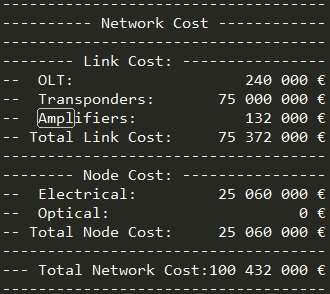
\includegraphics[width=8cm]{sdf/opaque/figures/script_opaque_surv_ref_high}
\caption{The ILP script used with the network cost.}
\label{scriptopaque_surv_ref_high}
\end{figure}


\subsection{Dimensioning using Heuristics}
\begin{tcolorbox}	
\begin{tabular}{p{2.75cm} p{0.2cm} p{10.5cm}} 	
\textbf{Student Name}  &:& Tiago Esteves    (October 03, 2017 - )\\
\end{tabular}
\end{tcolorbox}

\vspace{11pt}
In this section we will, again, do the dimensioning of the network mentioned in the first subsection to calculate the value of your CAPEX, for this we will use the Heuristic model describe in section \ref{heuristic_Opaque_Survivability} and we can get the best possible solution.
The software used to implement the above heuristics is Net2Plan.
In an initial phase will be described in a simple way how net2plan works, if a more complete description is necessary we can always consult the appendice \ref{net2planguide}, next will be presented the results for the scenarios mentioned previously.

\subsubsection{Net2Plan description}

In an initial phase we will have two aspects to fulfill. The first one is to define the ODU0, ODU1, ODU2, ODU3 and ODU4 matrices, and the second one passes through the design of the network in question.
After this phase is completed, we then apply the algorithms created. first the "joinTrafficMatrices" then the "logicalTopology" and finally the "Grooming".
At the end, the algorithm "CostReport" will be applied to obtain the CAPEX result for the network in question.

\subsubsection{Heuristics Results}

\textbf{Scenario 1: Reference Network Low Traffic}\\

Following all the steps mentioned in the previous subsection and using all the data referring to this scenario the obtained result can be consulted in the following table \ref{heuristicopaque_surv_ref_low}.

\begin{figure}[h!]
\centering
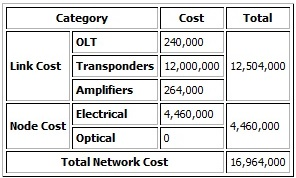
\includegraphics[width=9cm]{sdf/opaque/figures/heuristic_opaque_surv_ref_low}
\caption{The network cost using Net2Plan.}
\label{heuristicopaque_surv_ref_low}
\end{figure}


\textbf{Scenario 2: Reference Network High Traffic}\\

Following all the steps mentioned in the previous subsection and using all the data referring to this scenario the obtained result can be consulted in the following table \ref{heuristicopaque_surv_ref_high}.

\begin{figure}[h!]
\centering
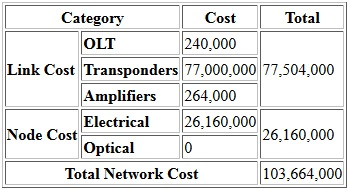
\includegraphics[width=9cm]{sdf/opaque/figures/heuristic_opaque_surv_ref_high}
\caption{The network cost using Net2Plan.}
\label{heuristicopaque_surv_ref_high}
\end{figure}


\subsection{Comparative Analysis}
\begin{tcolorbox}	
\begin{tabular}{p{2.75cm} p{0.2cm} p{10.5cm}} 	
\textbf{Student Name}  &:& Tiago Esteves    (October 03, 2017 - )\\
\end{tabular}
\end{tcolorbox}

\vspace{11pt}
In this subsection we will compare the CAPEX values obtained for the two scenarios in the three types of dimensioning. For a better analysis of the results will be created the table \ref{table_comparative_opaque_sur_ref_1} (scenario 1) and the table \ref{table_comparative_opaque_sur_ref_2} (scenario 2) with the different values obtained.\\

\textbf{Scenario 1:}\\

\begin{table}[h!]
\centering
\begin{tabular}{| c | c | c | c |}
 \hline
   & Analytical & ILP & Heuristic \\
 \hline\hline
 Link Cost & 16 372 000 \euro & 11 372 000 \euro & 12 504 000 \euro \\
 Node Cost & 5 125 500 \euro & 3 260 000 \euro & 4 460 000 \euro \\
 CAPEX & \textbf{21 497 500 \euro} & \textbf{14 632 000 \euro} & \textbf{16 964 000 \euro} \\
 \hline
\end{tabular}
\caption{Table with different value of CAPEX }
\label{table_comparative_opaque_sur_ref_1}
\end{table}

\vspace{11pt}
Looking at the previous table we can make some comparisons between the several different models of dimensioning and finally draw some conclusions.

\begin{itemize}
  \item We can conclude that in this case the dimensioning using ILP is the best (lowest cost).
  \item In comparison with the analytical model we can see that there is a difference considered with a 32\% error, this value is mainly due to the number of optical channels because in the analytical model more optical channels are calculated and used than those required in the ILP model.
  \item In comparison with the heuristic model we can see that there is a small difference with a 14\% error, much smaller than the previous one.
\end{itemize}

\vspace{11pt}
\textbf{Scenario 2:}\\

\begin{table}[h!]
\centering
\begin{tabular}{| c | c | c | c |}
 \hline
   & Analytical & ILP & Heuristic \\
 \hline\hline
 Link Cost & 160 372 000 \euro & 75 372 000 \euro & 77 504 000 \euro \\
 Node Cost & 8 453 250 \euro & 25 060 000 \euro & 26 160 000 \euro \\
 CAPEX & \textbf{168 825 250 \euro} & \textbf{100 432 000 \euro} & \textbf{103 664 000 \euro} \\
 \hline
\end{tabular}
\caption{Table with different value of CAPEX }
\label{table_comparative_opaque_sur_ref_2}
\end{table}

\vspace{11pt}
Looking at the previous table we can make some comparisons between the several different models of dimensioning and finally draw some conclusions.

\begin{itemize}
  \item We can conclude that in this case the dimensioning using ILP is the best (lowest cost).
  \item In comparison with the analytical model we can see that there is a difference considered with a 66\% error.
  \item In comparison with the heuristic model we can see that there is a smaller difference with a 3\% error.
\end{itemize}

